\subsection{Extensión: bonificación por sobrecumplimiento}

Esta subsección extiende el esquema \(B\) mediante el reconocimiento acotado de resultados superiores a las metas y una bonificación destinada al financiamiento de inversiones. El esquema \(B^{+}\) mantiene la tecnología, los márgenes de decisión y la estructura sancionadora de \(B\): el gerente continúa eligiendo únicamente los esfuerzos de ejecución \(e_r\) y eficiencia \(g_r\), mientras que las obligaciones de \(J^{G}\) y \(J^{F}\) conservan sus mecanismos específicos de verificación y consecuencia. La modificación aparece una vez alcanzadas las metas de \(J^{S}\): dentro de un rango predeterminado, un resultado adicional elegible puede continuar generando un retorno reputacional y un reconocimiento económico cuyos recursos permanecen afectados al financiamiento de inversiones. Como el conjunto de metas de servicio no cambia respecto de \(B\), la extensión conserva la ponderación individual \(1/n_S\) establecida para los indicadores de \(J^{S}\).

La bonificación no constituye ingreso directo del gerente ni recursos de libre disposición de la empresa. Su efecto sobre la utilidad gerencial opera a través de la valoración reputacional de los recursos reconocidos. Tampoco se incrementa la severidad sancionadora por estado. En particular,

\begin{subequations}
\label{eq:regla_sancionadora_bplus}
\begin{align}
M^{B^{+}}
&=
M^{B}
=
\mathrm{WACC}
\left(
B_S+B_G+B_F
\right),
\qquad
\chi^{B^{+}}=\chi^{B}=1,
\label{eq:multa_bplus}
\\
\mu_r^{B^{+}}
&=
\mu_r^{B},
\label{eq:exposicion_bplus}
\end{align}
\end{subequations}

donde las igualdades se refieren a un mismo estado regulatorio. Por tanto, el incentivo adicional de \(B^{+}\) proviene del reconocimiento del sobrecumplimiento y no de una mayor exposición sancionadora. Como el nuevo esquema puede modificar el esfuerzo óptimo y, con ello, los niveles de cumplimiento observados, \eqref{eq:regla_sancionadora_bplus} no implica necesariamente igualdad de las multas de equilibrio.

\subsubsection{Sobrecumplimiento reconocido y bonificación}

Las metas \(\bar q_j\) son predeterminadas por el regulador y no se derivan mecánicamente de la culminación de las inversiones. De acuerdo con \eqref{eq:produccion_calibracion_resultado}, un resultado \(q_j\) puede situarse por debajo, coincidir o superar su meta. Bajo \(B\), el cumplimiento \(c_j\) definido en la Subsección~4.1 se encuentra truncado en uno, por lo que una mejora adicional deja de modificar el ICG una vez alcanzada \(\bar q_j\). El esquema \(B^{+}\) extiende ese retorno dentro de un rango acotado.

Para cada \(j\in J^{S}\), sea \(\bar h_j>0\) el máximo sobrecumplimiento reconocido y \(\zeta_j\) un indicador de elegibilidad determinado por las condiciones establecidas ex ante. Se define

\begin{subequations}
\label{eq:sobrecumplimiento_bplus}
\begin{align}
\widetilde h_j
&\equiv
\min
\left\{
\max\left\{q_j-\bar q_j,0\right\},
\bar h_j
\right\},
\label{eq:sobrecumplimiento_potencial_bplus}
\\
\zeta_j
&\in
\{0,1\},
\label{eq:elegibilidad_bplus}
\\
h_j
&\equiv
\zeta_j\widetilde h_j.
\label{eq:sobrecumplimiento_reconocido_bplus}
\end{align}
\end{subequations}

El indicador \(\zeta_j\) toma el valor uno únicamente cuando el resultado adicional: i) puede verificarse con la misma periodicidad y trazabilidad que la meta base; ii) es atribuible a intervenciones o decisiones reconocidas por el regulador; iii) preserva las condiciones de calidad, capacidad y sostenibilidad exigibles; y iv) no se obtiene mediante recursos destinados a obligaciones pendientes. Si alguna condición falla, \(\zeta_j=0\). Así, \(h_j\) es nulo cuando no existe sobrecumplimiento elegible, aumenta con \(q_j\) dentro del rango reconocido y queda acotado en \(\bar h_j\). Las comparaciones marginales posteriores se realizan dentro de una región en la que \(\zeta_j\) permanece constante; un cambio en su valor constituye un cambio de estado.

El rango reconocido debe ser compatible con las posibilidades físicas de las intervenciones asociadas con el resultado. Como \(F_r\leq\bar F_r\), la tecnología de la Subsección~4.1 implica

\begin{subequations}
\label{eq:factibilidad_sobrecumplimiento_bplus}
\begin{align}
q_j^{\max}
&\equiv
q_{j,0}(X_j)
+
\sum_{r\in R_j^{S}}
\beta_{rj}\bar F_r,
\label{eq:resultado_maximo_bplus}
\\
\bar q_j+\bar h_j
&\leq
q_j^{\max}.
\label{eq:compatibilidad_sobrecumplimiento_bplus}
\end{align}
\end{subequations}

La segunda condición impide reconocer un rango de sobrecumplimiento superior al resultado máximo compatible con la tecnología del modelo. En particular, si \(\bar q_j=q_j^{\max}\), no existe holgura tecnológica y necesariamente \(\bar h_j=0\); en ese caso, \(B^{+}\) no agrega un incentivo de sobrecumplimiento para la meta \(j\).

Como \(B^{+}\) conserva el mismo conjunto \(J^{S}\) que \(B\), la regla de promedio aritmético continúa asignando a cada indicador individual el peso \(1/n_S\). Para mantener la medida regulatoria separada de la señal reputacional, se define el ICG extendido como

\begin{equation}
\label{eq:cumplimiento_bplus}
ICG^{B^{+}}
=
C_S
+
\frac{1}{n_S}
\sum_{j\in J^{S}}
\frac{h_j}{\bar q_j}.
\end{equation}

Cuando no existe sobrecumplimiento elegible, \(ICG^{B^{+}}=ICG^B=C_S\); cuando existe, el índice puede superar uno dentro del rango acotado por \(\bar h_j\). El cumplimiento base \(C_S\) y el componente adicional permanecen identificados separadamente. En particular, un mayor resultado en una meta no compensa, a efectos de exigibilidad, el incumplimiento de otra ni impide la aplicación de la consecuencia correspondiente, pues desde \(B\) la activación de la multa no depende del nivel agregado del ICG. La señal reputacional correspondiente se define separadamente más adelante mediante \(P^{B^{+}}\), preservando la distinción entre ponderación regulatoria y valoración reputacional introducida en la Subsección~4.1.

Además del reconocimiento dentro del indicador agregado, \(B^{+}\) incorpora una bonificación económica. Sea \(b_j>0\) el costo unitario regulatorio utilizado en el programa de inversiones del estudio tarifario para valorar la inversión asociada con el resultado \(j\), y sea \(\kappa_j\in[0,1]\) la proporción reconocida por cada unidad adicional elegible. Ambos parámetros se determinan ex ante y no dependen del costo efectivo ex post. La bonificación individual y agregada son

\begin{subequations}
\label{eq:bonificacion_bplus}
\begin{align}
T_j
&=
\kappa_j b_j h_j,
\label{eq:premio_individual}
\\
T
&=
\sum_{j\in J^{S}}T_j.
\label{eq:premio_agregado}
\end{align}
\end{subequations}

Por construcción, la bonificación es nula hasta alcanzar la meta, aumenta a una tasa \(\kappa_jb_j\) dentro del rango reconocido y queda acotada en \(\kappa_jb_j\bar h_j\). El estudio tarifario determina \(b_j\), \(\kappa_j\) y \(\bar h_j\), incluida la compatibilidad física de \eqref{eq:compatibilidad_sobrecumplimiento_bplus}. La calibración debe verificar ex ante la holgura tecnológica, la adicionalidad y trazabilidad del resultado, el costo regulatorio neto de la bonificación y el riesgo de desplazar recursos desde obligaciones pendientes.

\begin{figure}[!t]
    \centering
    \caption{Bonificación por sobrecumplimiento y límite del resultado reconocido}
    \label{fig:bonificacion_sobrecumplimiento}

    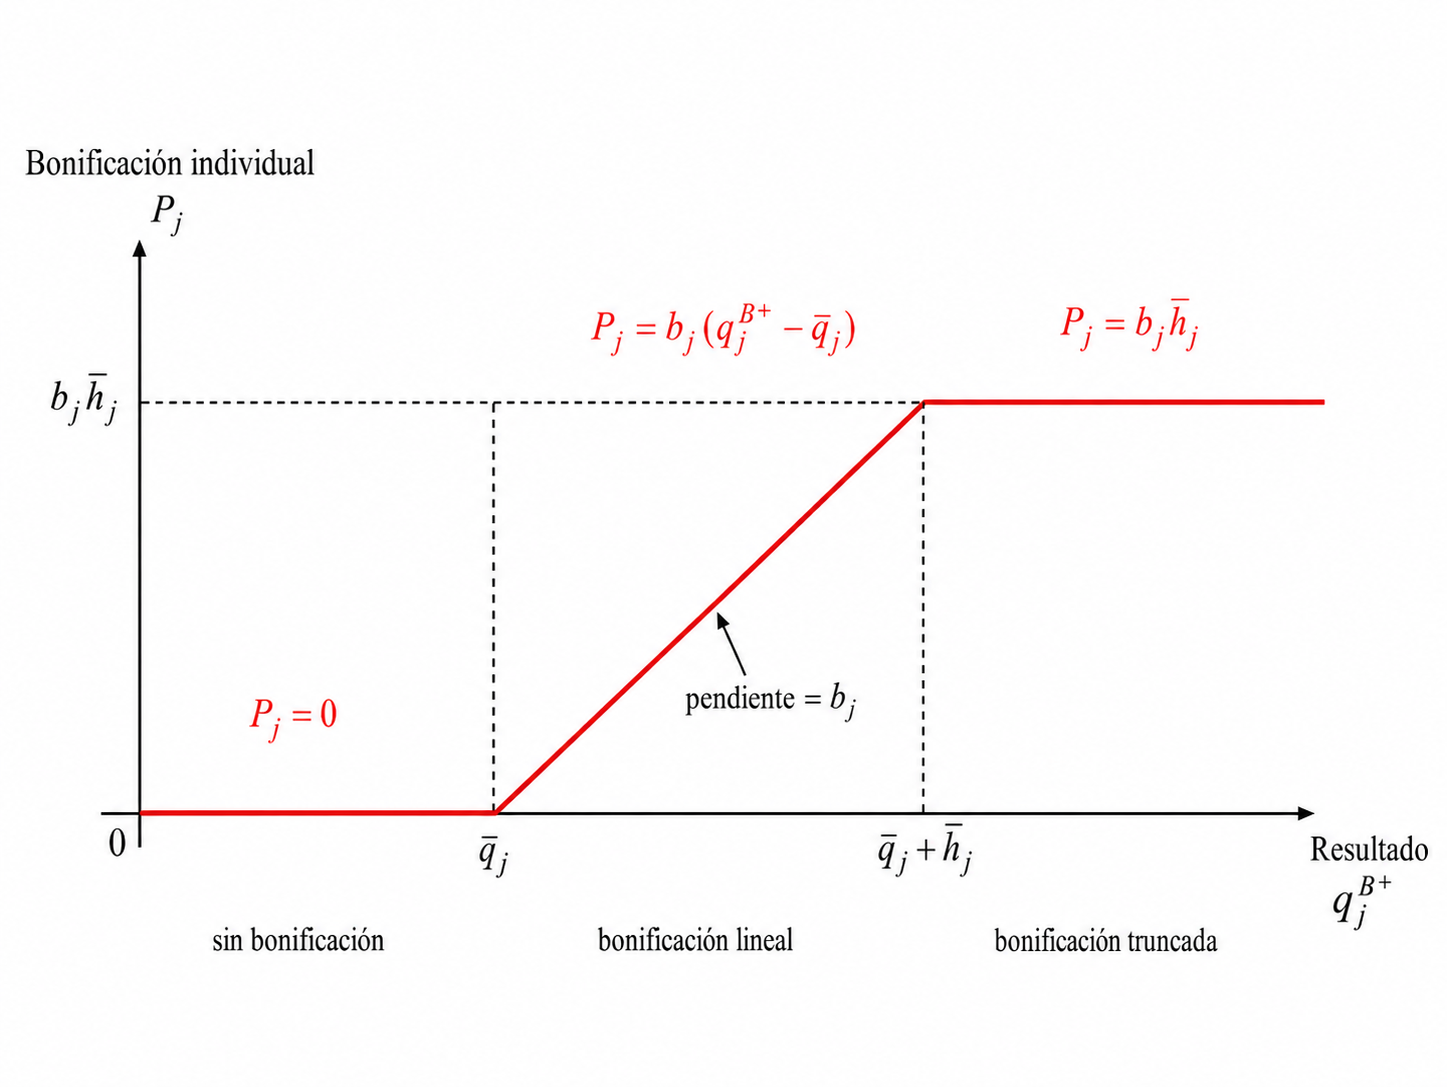
\includegraphics[width=\columnwidth]{figuras/bonif_sobrecumpl.png}

    \vspace{1mm}

    \begin{minipage}{\columnwidth}
        \raggedright
        {\footnotesize
        \textit{Nota:} Para un resultado elegible, la bonificación es nula hasta alcanzar la meta \(\bar q_j\), aumenta dentro del rango reconocido a una tasa \(\kappa_jb_j\) por unidad adicional y queda acotada en \(\kappa_jb_j\bar h_j\). Los parámetros \(b_j\), \(\kappa_j\) y \(\bar h_j\) se determinan ex ante en el estudio tarifario, sujeto a \(\bar q_j+\bar h_j\leq q_j^{\max}\).
        \textit{Fuente:} Elaboración propia.\par}
    \end{minipage}
\end{figure}

El monto reconocido mediante \(T\) se incorpora tarifariamente y permanece afectado al financiamiento de inversiones. Para evitar una doble contabilización, \(S^{B^{+}}\) recoge los recursos que permanecen efectivamente sin utilizar después de ejecutar el alcance que genera el resultado observado, mientras que \(T\) representa el reconocimiento regulatorio asociado con el sobrecumplimiento. Los recursos utilizados para producir el resultado adicional no se contabilizan simultáneamente como ahorro. En el canal reputacional, ambas formas de valor reconocido se consideran conjuntamente mediante \(R_E(S^{B^{+}}+T)\).

\subsubsection{Reputación e incentivo de ejecución bajo \(B^{+}\)}

El esquema \(B^{+}\) conserva las reglas de fiscalización y sanción de \(B\). Las metas de \(J^{G}\) y los indicadores específicos asociados con \(R^{F}\) permanecen fuera del ICG y mantienen sus mecanismos propios de verificación. La modificación se limita al reconocimiento acotado de resultados superiores a las metas.

Se supone que \(T\) no es apropiable por el gerente y no entra como compensación monetaria directa en \(U_G^{B^{+}}\). Su efecto opera únicamente a través de la valoración reputacional de los recursos reconocidos. Como \(B\) concentra la señal publicada en los resultados del servicio, el desempeño percibido bajo la extensión se define como

\begin{equation}
\label{eq:desempeno_percibido_bplus}
P^{B^{+}}
\equiv
C_S
+
\frac{1}{n_S}
\sum_{j\in J^{S}}
\frac{h_j}{\bar q_j}.
\end{equation}

Así, \(P^{B^{+}}=P^B=C_S\) cuando no existe sobrecumplimiento elegible. La reputación se extiende como

\begin{equation}
\label{eq:reputacion_bplus}
\begin{aligned}
\mathrm{Rep}^{B^{+}}
={}&
d_I\ell_I^{B^{+}}
R_I\left(P^{B^{+}}\right)
\\
&+
d_E\ell_E
R_E\left(S^{B^{+}}+T\right)
\\
&-
p\,d_M\ell_M
R_M\left(M^{B^{+}}\right).
\end{aligned}
\end{equation}

Si el regulador publica separadamente el cumplimiento base y el sobrecumplimiento reconocido, se supone \(\ell_I^{B^{+}}=\ell_I^{B}\). Los retornos marginales relevantes para los nuevos canales son

\begin{subequations}
\label{eq:retornos_marginales_bplus}
\begin{align}
\lambda^{B^{+}}
&\equiv
V'\!\left(\mathrm{Rep}^{B^{+}}\right)
d_I\ell_I^{B^{+}}
\notag\\
&\quad\times
R_I'\!\left(P^{B^{+}}\right),
\\
\varpi^{B^{+}}
&\equiv
V'\!\left(\mathrm{Rep}^{B^{+}}\right)
d_E\ell_E
\notag\\
&\quad\times
R_E'\!\left(S^{B^{+}}+T\right).
\label{eq:varpi_bplus}
\end{align}
\end{subequations}

Para aislar el efecto propio del sobrecumplimiento se mantienen localmente constantes los canales sancionadores comunes a ambos esquemas, de modo que \(\gamma^{B^{+}}=\gamma^{B}\). Las comparaciones se realizan dentro de una región en la que \(\zeta_j\) y los demás indicadores discretos permanecen fijos.

Considérese una intervención \(r\in R_j^{S}\). Mientras \(q_j\leq\bar q_j\), \(B^{+}\) coincide con \(B\) respecto del resultado \(j\). La diferencia aparece cuando \(\zeta_j=1\) y \(\bar q_j<q_j<\bar q_j+\bar h_j\). En ese intervalo,

\begin{subequations}
\label{eq:derivadas_sobrecumplimiento_bplus}
\begin{align}
\frac{\partial P^{B^{+}}}{\partial e_r}
&=
\frac{1}{n_S}
\frac{\beta_{rj}}{\bar q_j}
\notag\\
&\quad\times
\frac{\partial F_r}{\partial e_r}
>0,
\label{eq:derivada_p_bplus}
\\
\frac{\partial T}{\partial e_r}
&=
\kappa_j b_j
\beta_{rj}
\notag\\
&\quad\times
\frac{\partial F_r}{\partial e_r}
>0.
\label{eq:derivada_premio_bplus}
\end{align}
\end{subequations}

Para una intervención aún no culminada, \(\partial S_r/\partial e_r=0\). Como la regla sancionadora es común a \(B\) y \(B^{+}\), la diferencia entre los componentes continuos del beneficio marginal de ejecución es

\begin{equation}
\label{eq:incentivo_marginal_bplus}
\begin{aligned}
\mathrm{BM}_{r,e}^{B^{+}}
-
\mathrm{BM}_{r,e}^{B}
&=
\Biggl[
\lambda^{B^{+}}
\frac{1}{n_S\bar q_j}
\\
&\qquad
+
\varpi^{B^{+}}
\kappa_j b_j
\Biggr]
\beta_{rj}
\frac{\partial F_r}{\partial e_r}
\\
&\geq
0.
\end{aligned}
\end{equation}

El primer término recoge el retorno reputacional de reconocer el sobrecumplimiento dentro de \(P^{B^{+}}\) y el segundo la valoración reputacional de la bonificación destinada al financiamiento de inversiones. Ninguno requiere aumentar \(\mu_r^m\). La desigualdad es estricta cuando al menos uno de los nuevos canales tiene valoración positiva y la magnitud física continúa respondiendo al esfuerzo. Una vez alcanzado \(q_j\geq\bar q_j+\bar h_j\), \(h_j\) y \(T_j\) permanecen constantes y estos retornos marginales desaparecen.

La saturación del avance físico sí limita este mecanismo. Mientras \(e_r<e_r^{\mathrm{sat}}\), una mayor ejecución puede elevar \(F_r\), \(q_j\) y el sobrecumplimiento reconocido. Una vez alcanzada la región \(e_r\geq e_r^{\mathrm{sat}}\), \(\partial F_r/\partial e_r=0\) y los retornos marginales de \eqref{eq:derivadas_sobrecumplimiento_bplus} desaparecen por este canal.

\begin{resultadobox}
{Incentivo de ejecución bajo \(B^{+}\)}
\label{res:incentivo_ejecucion_bplus}

Para una intervención \(r\in R_j^{S}\), \(B^{+}\) no reduce el beneficio marginal de ejecución respecto de \(B\). Antes de alcanzar la meta ambos esquemas coinciden; dentro del rango de sobrecumplimiento elegible, \(B^{+}\) añade los retornos reputacional y económico asociados con el resultado adicional. Bajo la comparativa estática de la Subsección~4.1,

\begin{equation}
e_r^{B^{+},*}
\geq
e_r^{B,*}.
\end{equation}

La desigualdad es estricta cuando el reconocimiento modifica efectivamente el margen relevante de decisión, al menos uno de los canales adicionales tiene valoración positiva y la magnitud física continúa respondiendo al esfuerzo. El resultado no requiere una mayor exposición sancionadora que en \(B\).
\end{resultadobox}

\subsubsection{Eficiencia y uso de los recursos}

El esfuerzo de eficiencia \(g_r\) reduce los recursos necesarios para ejecutar una magnitud física dada, pero no eleva directamente \(F_r\), \(q_j\) ni el sobrecumplimiento reconocido cuando \(e_r\) permanece constante. Por tanto, el nuevo canal introducido por \(B^{+}\) no altera directamente el retorno tecnológico de \(g_r\).

Para una intervención completada, y manteniendo localmente constantes el resultado observado y \(T\),

\begin{equation}
\label{eq:incentivo_eficiencia_bplus}
\begin{aligned}
\frac{\partial (S^{B^{+}}+T)}{\partial g_r}
&=
-
\frac{\partial I_r}{\partial g_r}
>0,
\\
\mathrm{BM}_{r,g}^{B^{+}}
&=
\varpi^{B^{+}}
\left(
-
\frac{\partial I_r}{\partial g_r}
\right).
\end{aligned}
\end{equation}

El posible efecto intertemporal de los recursos liberados se rige por el canal descrito en la Subsección~4.3 y no constituye un efecto tecnológico directo de \(g_r\) sobre \(q_j\). Asimismo, como la bonificación se determina mediante parámetros fijados ex ante y a partir del resultado verificable, un mayor gasto no constituye por sí mismo una fuente de mayor reconocimiento.

\subsubsection{Desempeño bajo \(B^{+}\)}

El esquema \(B^{+}\) utiliza la misma función de producción de resultados que \(B\). Cualquier diferencia de desempeño proviene, por tanto, de los incentivos adicionales introducidos por el reconocimiento acotado del sobrecumplimiento y no de una modificación tecnológica ni de una mayor exposición sancionadora.

Bajo las condiciones locales del Resultado~\ref{res:incentivo_ejecucion_bplus}, si la respuesta inducida satisface \(F_r^{B^{+}}\geq F_r^{B}\) para las intervenciones relevantes de \(R^{S}\), la monotonicidad de la función de producción implica el siguiente resultado.

\begin{resultadobox}
{Desempeño bajo \(B^{+}\)}
\label{res:desempeno_bplus}

Bajo las condiciones locales anteriores,

\begin{equation}
\widetilde q_S^{B^{+}}
\geq
\widetilde q_S^{B}.
\end{equation}

La desigualdad es estricta cuando el reconocimiento del sobrecumplimiento induce una mayor ejecución física en al menos una intervención de \(R^{S}\) que contribuye positivamente al resultado correspondiente, sin una reducción compensatoria del desempeño generado por las demás intervenciones. Como \(B^{+}\) no modifica directamente los incentivos sobre \(R^{G}\) y la capacidad gerencial no es una restricción vinculante, se mantiene localmente \(C_G^{B^{+}}=C_G^{B}\). Por tanto,

\begin{equation}
\begin{aligned}
Q^{B^{+}}
&=
Q\!\left(
\widetilde q_S^{B^{+}},
C_G^{B}
\right)
\\
&\geq
Q\!\left(
\widetilde q_S^{B},
C_G^{B}
\right)
=
Q^{B}.
\end{aligned}
\end{equation}
\end{resultadobox}

\subsubsection{Bienestar regulatorio y calibración de la bonificación}

El mayor desempeño potencial de \(B^{+}\) no implica por sí solo una mejora de bienestar. A los componentes definidos en la Subsección~4.3 para una transición \(m\to m'\) se añade ahora el costo regulatorio neto de financiar la bonificación. Sea \(C_T(T)\) dicho costo, con

\begin{equation}
\label{eq:costo_bonificacion_bplus}
C_T(0)=0,
\qquad
C_T'(T)>0.
\end{equation}

La función \(C_T(T)\) recoge únicamente el costo fiscal, financiero o administrativo adicional de otorgar la bonificación, neto de su componente de transferencia, y excluye el gasto de inversión ya incorporado en \(C_I^{B^{+}}\). El caso \(C_T(T)=T\) solo corresponde cuando cada unidad reconocida constituye un costo adicional íntegro y distinto de los recursos contabilizados en \(C_I^{B^{+}}\).

El criterio regulatorio bajo \(B^{+}\) es

\begin{equation}
\label{eq:bienestar_regulador_bplus}
W_R^{B^{+}}
=
\Phi\!\left(
Q^{B^{+}}
\right)
-
C_I^{B^{+}}
-
C_{OM}^{B^{+}}
-
\Omega\!\left(M^{B^{+}}\right)
-
C_T(T),
\end{equation}

donde

\begin{equation}
Q^{B^{+}}
=
Q\!\left(
\widetilde q_S^{B^{+}},
C_G^{B^{+}}
\right).
\end{equation}

Utilizando las definiciones generales de \(\Delta_\Phi^{m,m'}\), \(\Delta_\Omega^{m,m'}\), \(\Delta_I^{m,m'}\) y \(\Delta_{OM}^{m,m'}\) de la Subsección~4.3, se añade

\begin{equation}
\label{eq:delta_p_bplus}
\Delta C_T^{B,B^{+}}
\equiv
C_T(T).
\end{equation}

La diferencia de bienestar se reduce entonces a

\begin{equation}
\label{eq:diferencia_bienestar_bplus_b}
\begin{aligned}
W_R^{B^{+}}
-
W_R^{B}
&=
\Delta_{\Phi}^{B,B^{+}}
+
\Delta_{\Omega}^{B,B^{+}}
\\
&\quad
-
\Delta_{I}^{B,B^{+}}
-
\Delta_{OM}^{B,B^{+}}
-
\Delta C_T^{B,B^{+}}.
\end{aligned}
\end{equation}

La igualdad \(M^{B^{+}}=M^B\) de \eqref{eq:multa_bplus} se refiere a un mismo nivel de cumplimiento. En equilibrio, el mayor esfuerzo inducido por \(B^{+}\) puede reducir las bases sancionadoras y, con ello, generar \(\Delta_\Omega^{B,B^{+}}\geq0\). Este canal puede reforzar la ganancia de bienestar, pero no es necesario para que la extensión resulte preferible.

De \eqref{eq:diferencia_bienestar_bplus_b}, la condición para una mejora regulatoria es

\begin{equation}
\label{eq:condicion_bienestar_bplus}
\Delta_{\Phi}^{B,B^{+}}
+
\Delta_{\Omega}^{B,B^{+}}
>
\Delta_{I}^{B,B^{+}}
+
\Delta_{OM}^{B,B^{+}}
+
\Delta C_T^{B,B^{+}}.
\end{equation}

\begin{resultadobox}
{Bienestar regulatorio bajo \(B^{+}\)}
\label{res:bienestar_bplus}

El hecho de que \(Q^{B^{+}}\geq Q^{B}\) no implica, por sí solo, que \(B^{+}\) domine a \(B\). Si se cumple \eqref{eq:condicion_bienestar_bplus}, entonces

\begin{equation}
W_R^{B^{+}}
>
W_R^{B}.
\end{equation}

Por tanto, \(B^{+}\) constituye una mejora regulatoria únicamente cuando el valor del sobrecumplimiento inducido y de cualquier reducción de la carga efectiva de la multa supera el costo neto de la bonificación y cualquier incremento del gasto de inversión o de los costos de operación y mantenimiento.
\end{resultadobox}

La condición de bienestar proporciona una interpretación económica para la calibración de \(\kappa_j\) y \(\bar h_j\). Un reconocimiento demasiado bajo puede no modificar suficientemente el esfuerzo, mientras que uno excesivamente alto puede elevar \(\Delta C_T^{B,B^{+}}\) por encima del valor regulatorio del desempeño adicional. El límite \(\bar h_j\) evita además que el mecanismo continúe reconociendo resultados una vez agotado el rango que el regulador considera valioso.

La incorporación de \(B^{+}\) al ordenamiento condicionado completo de bienestar se presenta en la Subsección~4.5.
